\documentclass{article}
\usepackage[utf8]{inputenc}
\usepackage{amsfonts,amsthm,amsmath,amssymb,mathtools}
\usepackage{tikz}
\usetikzlibrary{arrows,backgrounds,matrix,positioning,shapes.geometric,
shapes.misc,calc,patterns}
\usepackage[]{xcolor}

\begin{document}

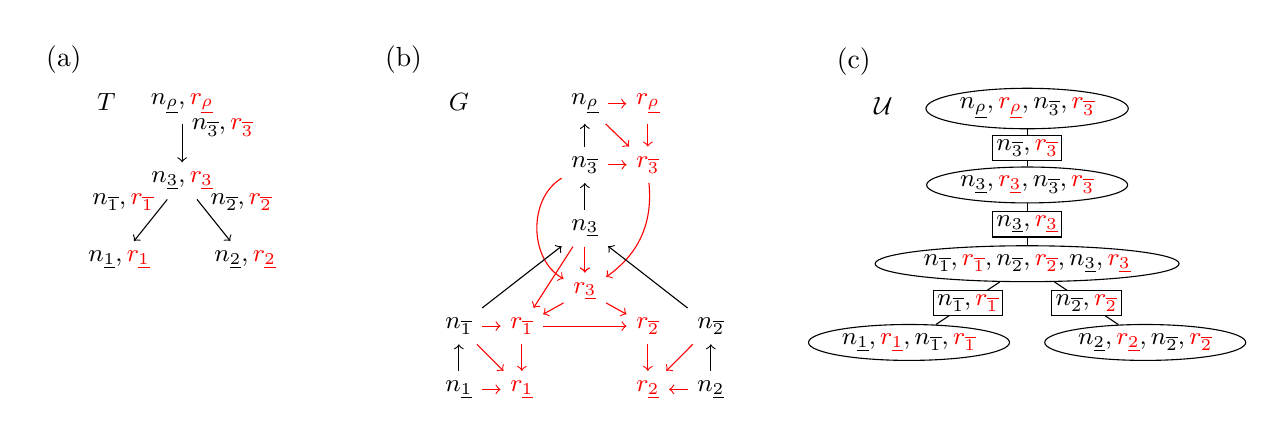
\begin{tikzpicture}[-]
\matrix (m0)[matrix,anchor=north,
        column sep={0.8cm,between origins},
        row sep={1cm,between origins},
        nodes={font=\small}] at (0,0)
{\node[label={[xshift=-2em]:\normalsize (a)}](){\hspace{-1em}$T$}; &
\node(x0){$n_{\underline{\rho}},\textcolor{red}{r_{\underline{\rho}}}$}; & \\
& \node(x3){$n_{\underline{3}},\textcolor{red}{r_{\underline{3}}}$}; & \\
\node(x1){$n_{\underline{1}},\textcolor{red}{r_{\underline{1}}}$}; & &
\node(x2){$n_{\underline{2}},\textcolor{red}{r_{\underline{2}}}$}; \\
};

\matrix (m1)[matrix,anchor=north,
    column sep={8mm,between origins},
    row sep={8mm,between origins},
    nodes={font=\small}] at (5,0)
{\node[label={[xshift=-2em]:\normalsize (b)}]{$G$};
& & \node(n0b){$n_{\underline{\rho}}$}; & \node[red](r0b){$r_{\underline{\rho}}$}; & \\
& & \node(n3t){$n_{\overline{3}}$}; & \node[red](r3t){$r_{\overline{3}}$}; & \\
& & \node(n3b){$n_{\underline{3}}$}; & & \\
& & \node[red](r3b){$r_{\underline{3}}$}; & & \\[-1em]
\node(n1t){$n_{\overline{1}}$}; & \node[red](r1t){$r_{\overline{1}}$}; & &
\node[red](r2t){$r_{\overline{2}}$}; & \node(n2t){$n_{\overline{2}}$}; \\
\node(n1b){$n_{\underline{1}}$}; & \node[red](r1b){$r_{\underline{1}}$}; & &
\node[red](r2b){$r_{\underline{2}}$}; & \node(n2b){$n_{\underline{2}}$}; \\
};

\matrix (m2)[matrix,anchor=north,
    column sep={1.5cm,between origins},
    row sep={1cm,between origins},
    nodes={font=\small,ellipse,draw,inner sep=.5mm}] at (11,0)
{\node[draw=none,label={[xshift=-2em]:\normalsize (c)}](){\hspace{-2em}$\mathcal{U}$}; &
\node(c0b){$n_{\underline{\rho}},\textcolor{red}{r_{\underline{\rho}}},
n_{\overline{3}},\textcolor{red}{r_{\overline{3}}}$}; & \\
& \node(c3t){$n_{\underline{3}},\textcolor{red}{r_{\underline{3}}},
n_{\overline{3}},\textcolor{red}{r_{\overline{3}}}$}; & \\
& \node(c3b){$n_{\overline{1}},\textcolor{red}{r_{\overline{1}}},
n_{\overline{2}},\textcolor{red}{r_{\overline{2}}},
n_{\underline{3}},\textcolor{red}{r_{\underline{3}}}$}; & \\
\node(c1t){$n_{\underline{1}},\textcolor{red}{r_{\underline{1}}},
n_{\overline{1}},\textcolor{red}{r_{\overline{1}}}$}; & &
\node(c2t){$n_{\underline{2}},\textcolor{red}{r_{\underline{2}}},
n_{\overline{2}},\textcolor{red}{r_{\overline{2}}}$}; \\
};
\begin{scope}[every node/.style={font=\small\itshape}]
\draw[->] (x0) -- node[above right,
    yshift=-.1em]{$n_{\overline{3}},\textcolor{red}{r_{\overline{3}}}$}(x3);
\draw[->] (x3) -- node[left,above,
    xshift=-1em]{$n_{\overline{1}},\textcolor{red}{r_{\overline{1}}}$}(x1);
\draw[->] (x3) -- node[right,above,
    xshift=1em]{$n_{\overline{2}},\textcolor{red}{r_{\overline{2}}}$}(x2);

\draw[->,red] (n0b) -- (r0b);
\draw[->,red] (n0b) -- (r3t);
\draw[->,red] (r0b) -- (r3t);
\draw[->,red] (n3t) -- (r3t);
\draw[->] (n3t) -- (n0b);
\draw[->] (n3b) -- (n3t);
\draw[->,red,bend right=60] (n3t) to (r3b);
\draw[->,red] (n3b) -- (r3b);
\draw[->,red,bend left=30] (r3t) to (r3b);

\draw[->,red] (n1b) -- (r1b);
\draw[->] (n1b) -- (n1t);
\draw[->,red] (n1t) -- (r1t);
\draw[->,red] (r1t) -- (r1b);
\draw[->,red] (n1t) -- (r1b);
\draw[->,red] (n2b) -- (r2b);
\draw[->] (n2b) -- (n2t);
\draw[->,red] (r2t) -- (r2b);
\draw[->,red] (n2t) -- (r2b);
\draw[->] (n1t) -- (n3b);
\draw[->] (n2t) -- (n3b);
\draw[->,red] (n3b) -- (r3b);
\draw[->,red] (n3b) -- (r1t);
\draw[->,red] (r3b) -- (r1t);
\draw[->,red] (r3b) -- (r2t);
\draw[->,red] (r1t) -- (r2t);

\draw[-] (c1t) -- (c3b) node[midway,rectangle,draw,fill=white,
    inner sep=.5mm]{$n_{\overline{1}},\textcolor{red}{r_{\overline{1}}}$};
\draw[-] (c2t) -- (c3b) node[midway,rectangle,draw,fill=white,
    inner sep=.5mm]{$n_{\overline{2}},\textcolor{red}{r_{\overline{2}}}$};
\draw[-] (c3b) -- (c3t) node[midway,rectangle,draw,fill=white,
    inner sep=.5mm]{$n_{\underline{3}},\textcolor{red}{r_{\underline{3}}}$};
\draw[-] (c3t) -- (c0b) node[midway,rectangle,draw,fill=white,
    inner sep=.5mm]{$n_{\overline{3}},\textcolor{red}{r_{\overline{3}}}$};
\end{scope}
\end{tikzpicture}

\end{document}